\documentclass[a4paper,11pt,twocolumns]{article}
%\documentclass[dvips]{article}
\usepackage{graphicx}
\usepackage[spanish,activeacute]{babel}
\usepackage[margin=0.8in]{geometry}
\bibliographystyle{plain}
\usepackage{hyperref}
\usepackage{amssymb,amsmath}
\usepackage{draftwatermark}
\usepackage{graphicx}
\usepackage[normalem]{ulem}
\SetWatermarkFontSize{40pt}
\SetWatermarkScale{6}
\begin{document}

\twocolumn
\setlength{\columnsep}{25pt}

\title{Midiendo la Performance de SPDY}
\author{Pablo Maximiliano Lulic}

\maketitle

\begin{abstract} 
Actualmente, la Web se sustenta con el est'andar \textsc{http}. Este protocolo tuvo su 'ultima versi'on en el a'no 1999. L'as p'aginas en ese entonces eran muy diferentes a las actuales, tanto en contenido como en recursos. Google desarroll'o un protocolo en el a'no 2009 llamado \textsc{spdy}, cuyo prop'osito es mejorar la performance en la recuperaci'on de los recursos de la web. A pesar de su gran aceptaci'on y de sentar las bases del pr'oximo \textsc{http 2.0}, hay ciertas cuestiones que todav'ia quedan por revisar. En este paper, se propone evaluar la performance de \textsc{spdy} desde dos enfoques diferentes, uno en embientes espec'ificos y otro en la web.
\end{abstract}

\section{Introducci'on}

El protocolo \textsc{http} tuvo su primera versi'on en mayo de 1996, culminando en 1999 con el est'andar actual que es el \textsc{http}  1.1 \cite{rfcHTTP} Es un protocolo sin estado, el servidor no mantiene informaci'on acerca de las diferentes peticiones que le llegan, lo que conlleva a que se necesite realizar una conexi'on nueva por cada recurso que se necesite de un sitio web.

\section{La Web en la Actualidad}

En comparaci'on con lo que era la web en la 'epoca en la que se implement'o el protocolo \textsc{http}, hubo un crecimiento amplio en el tama'no y en la cantidad de recursos de un sitio web. Para Noviembre de 2013 \cite{httpArchive}, el tama'no promedio de un sitio era de 1614kb, en contraste con Noviembre de 2010 que el tama'no promedio era de 702kb, el aumento fue casi del 50\%. Estudios m'as recientes, indican que el crecimiento de un sitio promedio es del \%151 \cite{tammy} (ver figura \ref{average}).

\begin{figure}[h!]
  	\centering
	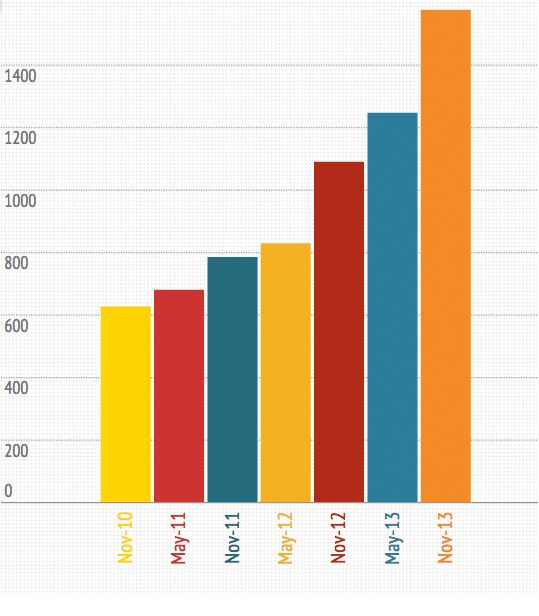
\includegraphics[scale=0.4]{151tammy}
	\caption{\small Crecimiento del tama'no de los sitios promedio, extra'ido de \cite{tammy}}
	\label{average}
\end{figure}

El crecimiento se produce con velocidad \cite{averageWebPage} y hay otras cuestiones relacionadas al tiempo de carga de una p'agina, no solo el ancho de banda \cite{moreBand}, sino por ejemplo, el \textsc{rtt}\footnote{Tiempo que tarda un paquete de datos en ir desde el emisor al receptor y volver al emisor.}, como se puede ver en la figura \ref{rttBelsche}

\begin{figure}[h!]
  	\centering
	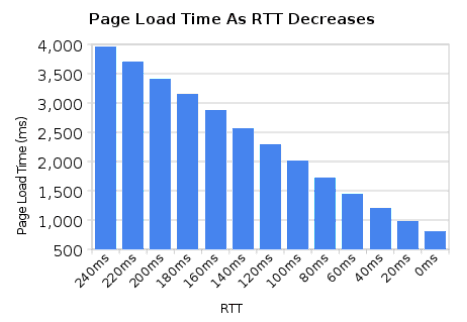
\includegraphics[scale=0.5]{belsche}
	\caption{\small Tiempo de carga de una p'agina mientras se var'ia el RTT, extra'ido de \cite{moreBand}}
	\label{rttBelsche}
\end{figure}

\section{SPDY}

\textsc{spdy}\cite{SPDYWhitepaper} es un protocolo de la capa de aplicaci'on \cite{illustratedTCPIP} que funciona sobre SSL \cite{rfcSSL}, permite la transmisi'on de Streams\footnote{???} sobre una conexi'on normal de \textsc{tcp}, que es el Protocolo de Control de Transmisi'on de la capa de Transporte \cite{illustratedTCPIP}). A continuaci'on se comentar'an las caracter'isticas del Protocolo (extra'idas de \cite{SPDYWhitepaper}):

\begin{enumerate}

\item Streams Multiplexados.

\item Priorizaci'on de Peticiones.

El Cliente puede tantos recursos como quiera del Servidor y asignarle prioridad a cada uno de ellos.

\item Compresi'on de los Headers \textsc{http} \cite{headersHTTP}.

Comprime los headers de petici'on y respuesta \textsc{http}.

\item Push

Permite al Servidor enviarle recursos al Cliente sin que este se lo pida.

\item Hint

Permite al Servidor ''sugerirle'' al Cliente que pida alg'un recurso espec'ifico.

\end{enumerate}

\section{Experimento 1}

\subsection{Preparaci'on}

Se virtualizaron 3 m'aquinas utilizando VirtualBox \cite{virtualBox}, disponibles para su descarga en \cite{maqVirtuales}.
Se dise'no la siguiente topolog'ia de Red:

\vspace*{1\baselineskip}
\begin{math}
\frac{\textbf{CLIENTE}}{Lubuntu 13.10 \cite{lubuntu}} \longleftrightarrow \frac{\textbf{PROXY}}{FreeBSD \cite{FreeBSD}}  \longleftrightarrow \frac{\textbf{SERVIDOR}}{Ubuntu Server 13.10 \cite{ubuntu}} 
\end{math}

\vspace*{1\baselineskip}

\begin{enumerate}
\item SERVIDOR

Se descargaron los sitios\footnote{Utilizando la opci'on ''Guardar como...'' de Google Chrome, que obtiene todos los recursos externos y los almacena en una carpeta.} y se configuraron los siguientes hosts virtuales en el Servidor:
\begin{enumerate}
\item www.amazon.com
\item www.bing.com
\item login.yahoo.com
\item www.world-flags.com \cite{flags}
\end{enumerate}
Cada sitio se brind'o utilizando Apache 2.2 \cite{apache}. En \textsc{http} plano, en \textsc{https} utilizando mod\_ssl \cite{modSSL} con un certificado SSL autofirmado con Ubuntu \cite[Secci'on 4]{spdyGT}, y para brindar \textsc{spdy}, se instal'o mod\_spdy \cite{modSPDY}. con el prop'osito de poder realizar un an'alisis de los paquetes que viajan luego de finalizado el experimento se realiz'o la siguiente modificaci'on en la configuraci'on del SSL, que es el archivo \emph{''/etc/apache2/mods-enabled/ssl.conf''} \cite{siffSSL}.

\begin{quote}\small
\#   SSL Cipher Suite:

\#   List the ciphers that the client is permitted to negotiate.

\#   See the mod\_ssl documentation for a complete list.

\#   enable only secure ciphers:

\sout{\#SSLCipherSuite HIGH:MEDIUM:!ADH:!MD5}

SSLCipherSuite DES-CBC3-SHA
\end{quote}

\item PROXY

Utilizando la herramienta Dummynet \cite{dummynet} que viene instalada en la distribuci'on de FreeBSD, se utilizaron diferentes comandos \cite{ipfw} para filtrar el tr'afico en la red\footnote{Ancho de Banda y Retardo.} y simular diferentes entornos. Se habilit'o la Dummynet modificando el archivo \emph{''/etc/rc.conf''} con las siguientes l'ineas

\begin{quote}\small
firewall\_enable=''YES''

firewall\_type=''OPEN''

gateway\_enable=''YES''
\end{quote}
Se configur'o el siguiente flag:
\begin{quote}\small
sysctl net.inet.ip.forwarding=1
\end{quote}
Y por 'ultimo, para que la Dummynet se cargue junto con el Kernel del BSD se agreg'o la siguiente l'inea en el archivo \emph{''/bot/loader.conf''}
\begin{quote}\small
dummynet\_load=''YES''
\end{quote}
\item CLIENTE

Se instal'o NodeJS \cite{nodeJS} y se descarg'o el software \emph{chrome-har-capturer} \cite{harCapt} de GitHub \cite{github}.
Se utiliz'o el navegador \emph{Chromium} Versi'on 30 que, a trav'ez de su API de depuraci'on remota \cite{debuggingChrome}, permite al \emph{chrome-har-capturer} interactuar con dicho navegador para poder navegar un sitio particular y obtener un archivo \emph{.har}\footnote{Archivo con notaci'on JSON \cite{json} que contiene la traza del Navegador Web con el sitio}, con los resultados de la interacci'on del navegador con el sitio. Tambi'en, fue utilizada la herramienta \emph{TShark}\cite{tshark} para poder capturar los paquetes que viajaron en la red durante el experimento.

\end{enumerate} 

\subsection{Metodolog'ia}

Con la idea de comparar los m'etodos \textsc{http}, \textsc{https} y \textsc{spdy} en diferentes ambientes simulados, se definieron los siguientes valores:

\vspace*{1\baselineskip}
\begin{tabular}{ l c r }
	Ancho de Banda (BW)  \\ \hline
  	100 Kbps \\
	256 Kbps \\
	512 Kbps \\
	1024 Kbps \\
	2048 Kbps \\
	5120 Kbps \\
	10240 Kbps \\
\end{tabular}
\vspace*{1\baselineskip}
\begin{tabular}{ l c r }
	Retraso (RTT) \\ \hline
  	10 ms \\
	50 ms \\
	100 ms \\
	200 ms \\
	250 ms \\
	500 ms \\
	\\
\end{tabular}

Estos valores, se iban configurando autom'aticamente en el Proxy mediante el siguiente comando:

\begin{quote}\small
comando
\end{quote}

Se combinaron todos los Anchos de Banda con todos los Retrasos para cada uno de los m'etodos por p'agina\footnote{Por ejemplo: 100Kbps de Ancho de Banda con 100ms de Retraso accediendo al host virtual de Amazon por \textsc{https} (https://www.amazon.com).}, se repiti'o el experimento 5 veces y se promediaron los resultados.

\subsection{Resultados}

SEGUIR ACA

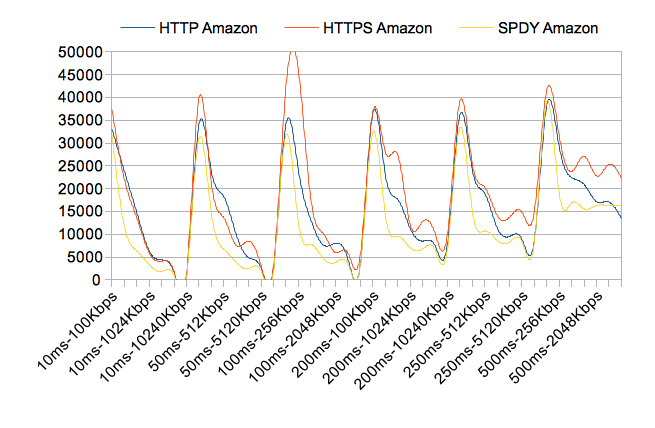
\includegraphics[scale=0.5]{res_amazon}

\section{Experimento 2}

\subsection{Preparaci'on}

\subsection{Metodolog'ia}

\subsection{Resultados}

\section{Conclusiones y Trabajos Relacionados}

\nocite{*}
\bibliography{bibliography}

\end{document}